\documentclass[conference]{IEEEtran}

\IEEEoverridecommandlockouts                              % This command is only needed if 
                                                          % you want to use the \thanks command

\overrideIEEEmargins                                      % Needed to meet printer requirements.

% See the \addtolength command later in the file to balance the column lengths
% on the last page of the document

\usepackage{amssymb}
\setcounter{tocdepth}{3}
\usepackage{graphicx}
\usepackage[fleqn]{amsmath}
\usepackage{url}
\usepackage{amsmath} % assumes amsmath package installed
\usepackage{amssymb}  % assumes amsmath package installed
\usepackage{algorithm}			% pacchetti per i pezzi di pseudocodice
\usepackage{algorithmic}		% pacchetti per i pezzi di pseudocodice

\usepackage{float}		% pacchetto per figure e tabelle


%\usepackage{mathptmx} % assumes new font selection scheme installed
%\usepackage{times} % assumes new font selection scheme installed


% correct bad hyphenation here
\hyphenation{op-tical net-works semi-conduc-tor}


\begin{document}
%
% paper title
% can use linebreaks \\ within to get better formatting as desired
\title{ART@Work: Team Description Paper}

\author{\IEEEauthorblockN{Marco Imperoli\IEEEauthorrefmark{1},
Michele Marostica\IEEEauthorrefmark{2},
Nicolò Boscolo\IEEEauthorrefmark{2}
Roberto Capobianco\IEEEauthorrefmark{1}
Jacopo Serafin\IEEEauthorrefmark{1}\\
Alberto Pretto\IEEEauthorrefmark{1},
Daniele Nardi\IEEEauthorrefmark{1} and
Enrico Pagello\IEEEauthorrefmark{2}}\\
\IEEEauthorblockA{\IEEEauthorrefmark{1}Department of Computer, Control, and Management Engineering\\``Antonio Ruberti``, Sapienza University of Rome, Italy.\\ Email: {\tt\small marcoimperoli@gmail.com, \{serafin,capobianco,pretto,nardi\}@dis.uniroma1.it}\\
Website: http://labrococo.dis.uniroma1.it}
\IEEEauthorblockA{\IEEEauthorrefmark{2}Department of Information Engineering, University of Padua, Italy.\\ Email: {\tt\small michelemaro@gmail.com, nicolo.boscolo@it-robotics.it, epv@dei.unipd.it}\\Website: http://robotics.dei.unipd.it}}

% make the title area
\maketitle


\begin{abstract}
%\boldmath
The ART@Work team, where ART is the acronym for Azzurra Robot Team, is a newly created team from the collaboration between the Cognitive Cooperating Robots laboratory of the Sapienza University of Rome and the Intelligent Autonomous Systems Laboratory of the University of Padua. \\
This document describes the scientific background, the team members' competencea, the research contribution and the performance improvements we expect to achieve before the 2014 RoCKIn competition event.
\end{abstract}


\section{Introduction}
% no \IEEEPARstart
[The following is just a test] The laboratory RoCoCo (Cognitive Cooperating Robots) is located at DIAG (Dipartimento di Ingegneria Informatica, Automatica e Gestionale) of Sapienza University of Rome, Italy.
The research developed at RoCoCo laboratory is in the area of Artificial Intelligence and Robotics. RoCoCo has been involved in RoboCup competitions since 1998 in different leagues: Middle-size 1998-2002, Four-legged 2000-2007, Real-rescue-robots 2003-2006, @Home in 2006, Virtual-rescue since 2006 and Stan-dard platform League (Nao Division) since 2008.\\
IAS-Lab stands for Intelligent Autonomous Systems Laboratory and it is one of the 28 laboratories of the Department of Information Engineering of the University of Padua.
The activity at IAS-Lab concerns the study of several fields of Robotics: computer vision, humanoids and wheeled robot programming, virtual simulation, biomechanical model based on human biosignal and wearable robots design for rehabilitation purposes.\\

Test citation \cite{thrunburgardfox2005}.\\

\subsection{Team Details}
\begin{itemize}
 \item \textbf{Team name:} ART@Work
 \item \textbf{Selected track:} RoCKIn@Work
 \item \textbf{Team leader:} XXX
 \item \textbf{Team members:} Marco Imperoli, Michele Marostica, Nicolò Boscolo, Roberto Capobianco, Jacopo Serafin
 \item \textbf{Team coordinator:} Alberto Pretto
 \item \textbf{Advisors:} Daniele Nardi and Enrico Pagello 
 \item \textbf{Robot:} 1 Kuka Youbot
\end{itemize}

\subsection{Competence of Team Members}
[Ognuno dovrebbe aggiungere uno short bio (massimo 2-3 frasi) che include le comptetenze principali]
\subsubsection{Marco Imperoli}
XXX
\subsubsection{Michele Marostica}
XXX
\subsubsection{Nicolò Boscolo}
XXX
\subsubsection{Roberto Capobianco}
XXX
\subsubsection{Jacopo Serafin}
XXX


\section{Robot Description}
Include an image of our robot, test Image in Fig.~\ref{fig:test_img}.\\
\begin{figure}[t!]
\begin{center}
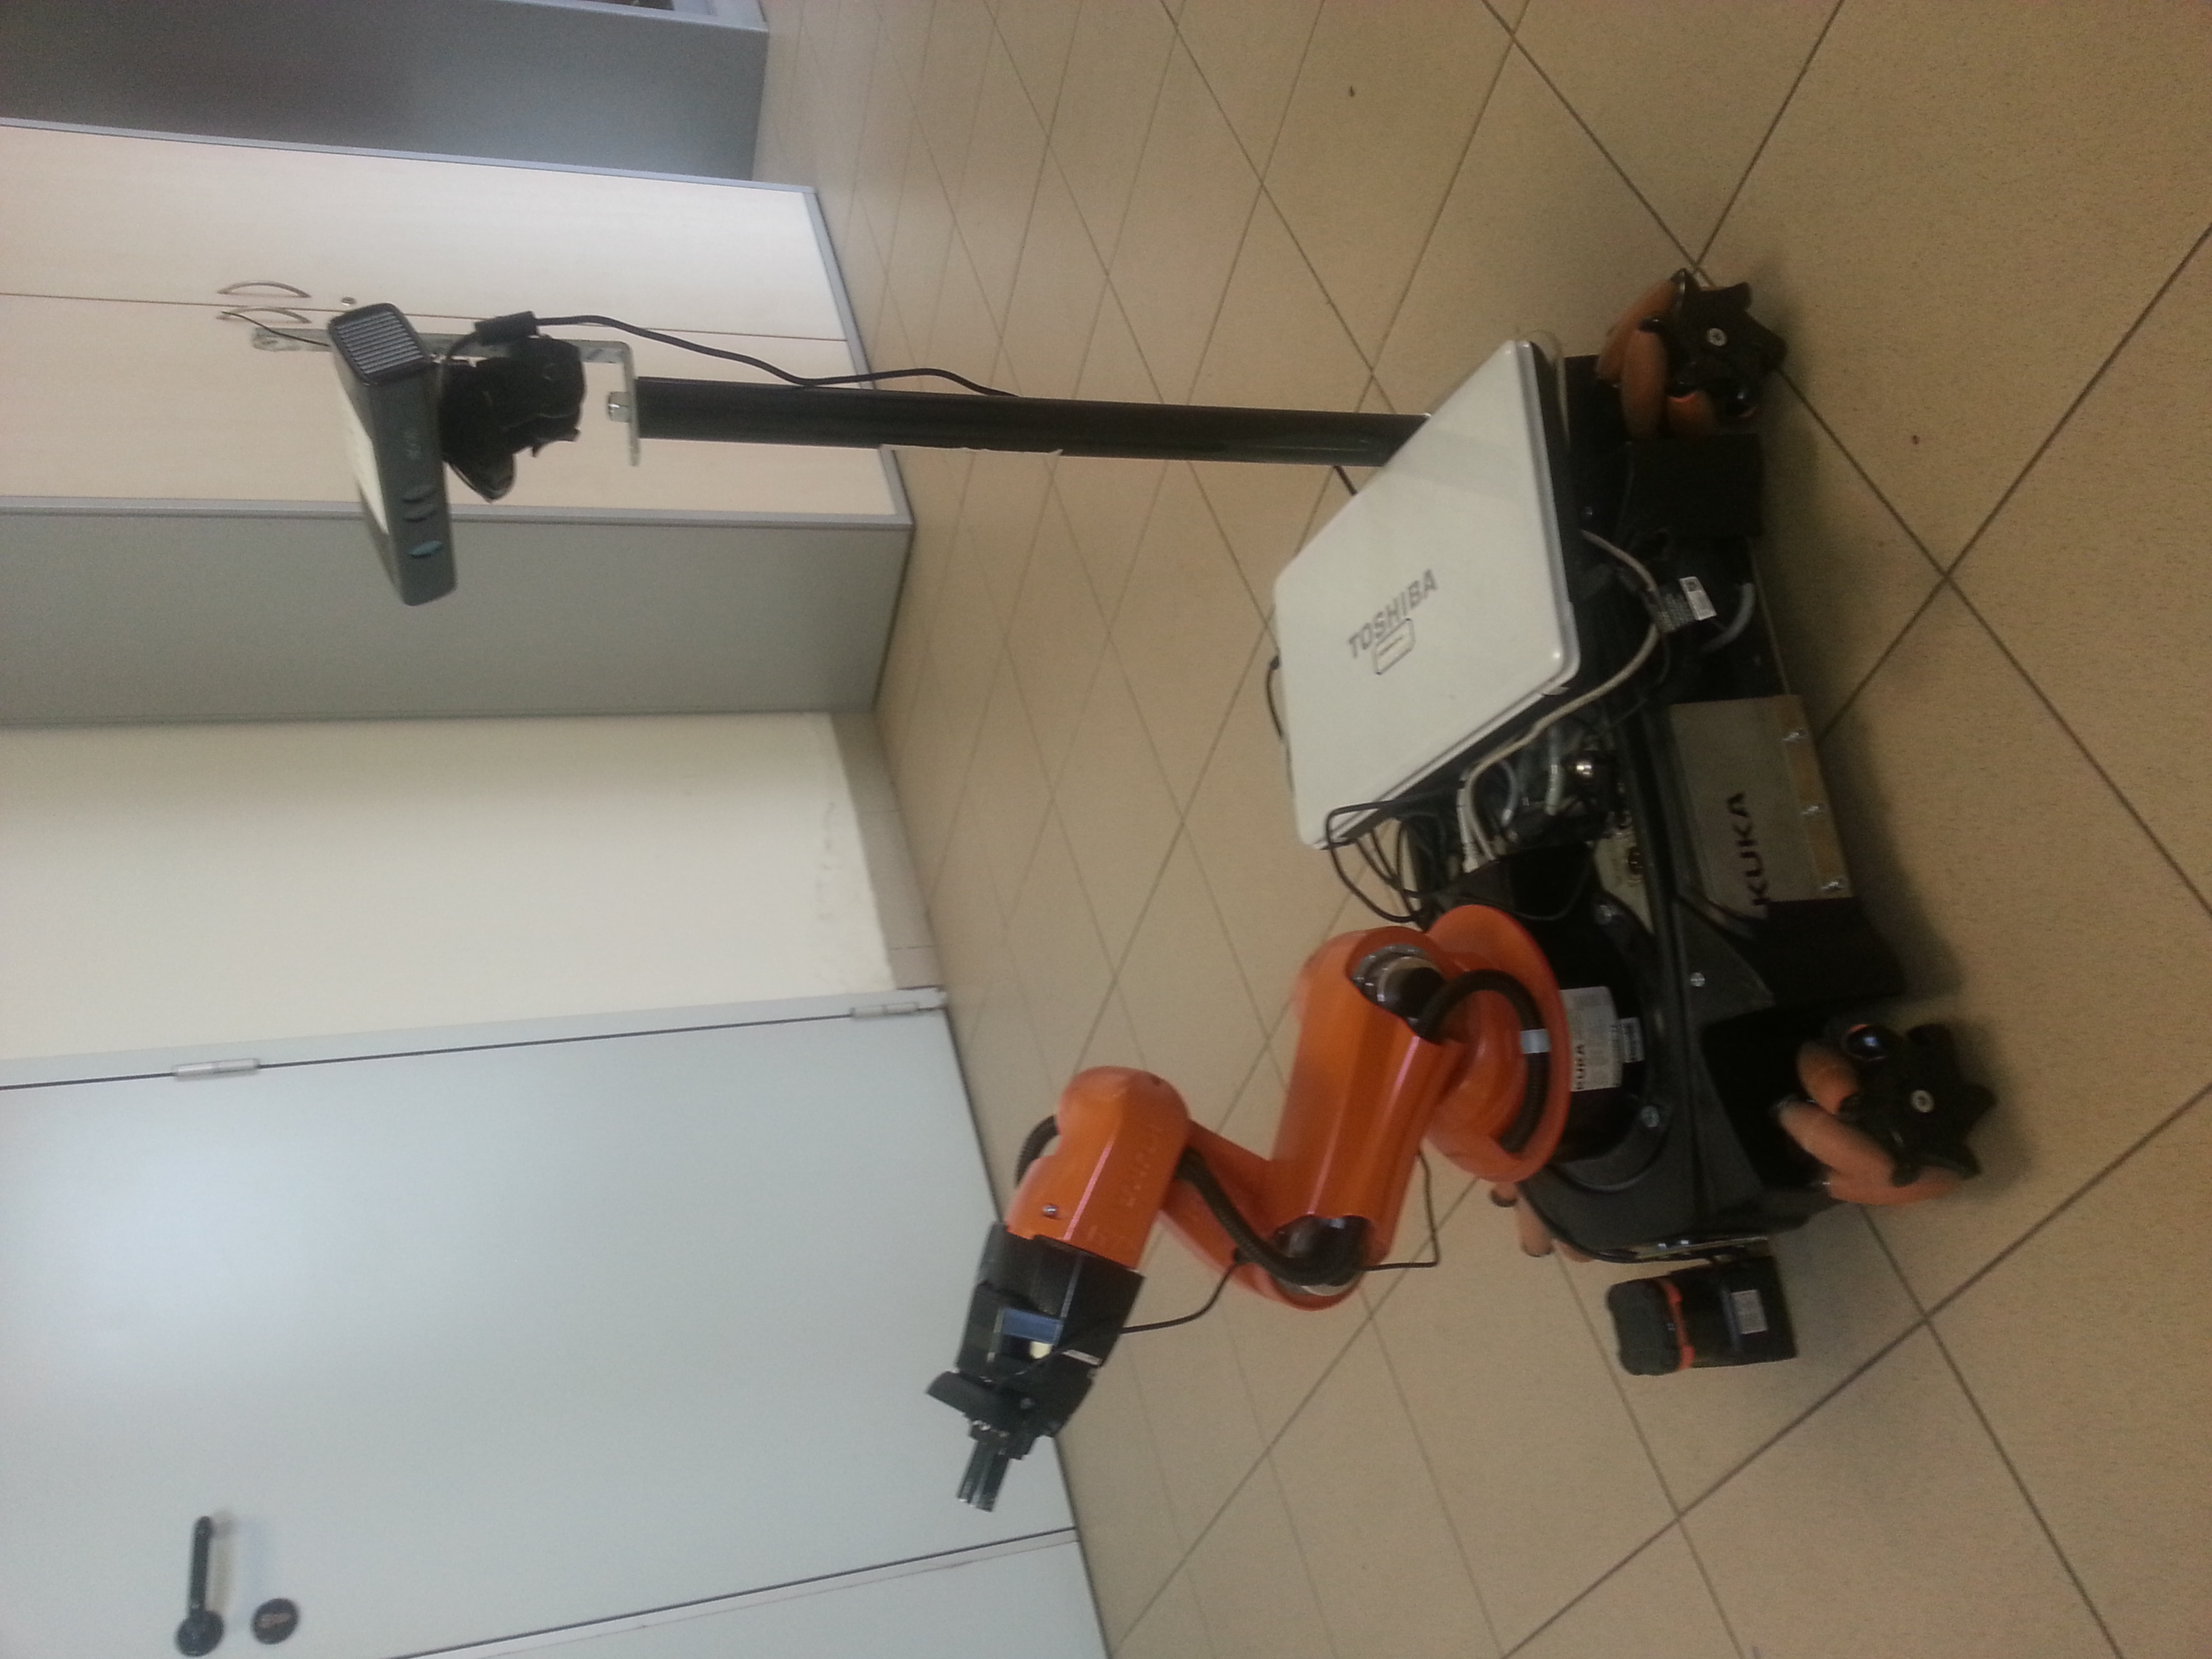
\includegraphics[angle=0,width=\linewidth]{images/test_img.png}
\end{center}
\caption{Test image.}\label{fig:test_img}
\end{figure}

\section{Software Infrastructure}
\subsubsection{Middleware}

\section{Research areas}

[Aggiungere una descrizione delle attività scientifiche/esperienza nell'ambito della robotica (ovvero, argomenti delle tesine, tesi, paper, eccc..). Chi ha paper pubblicati, dovrebbe citarsi, aggiungendo la entry nel file .bib.]

\section{Applicability and Relevance to Industrial Robotics}


\section{Conclusion}
Some brief conclusion

\bibliographystyle{IEEEtran}
\bibliography{bibliography} 

% that's all folks
\end{document}


